% !TEX root = ../main.tex
% --+ PHYSICS +-----------------------------------------------------------------
% TODO. Include a description of the 5 DIS variables we use.

% --+ 10.11 DIS +---------------------------------------------------------------
\begin{frame}{Deep Inelastic Scattering (DIS)}
    \label{10.11::dis}

    \begin{itemize}
        \item
            DIS refers to the scattering of an $e^-$ off a quark inside a nucleon.

        \item
            If we can detect the scattered $e^-$ and one of the scattered hadrons, we refer to the process as Semi Incluside DIS (SIDIS).
    \end{itemize}

    \vspace{-12pt}
    \begin{columns}[onlytextwidth,T]

    \begin{column}{.49\linewidth}
        \begin{center}
            \begin{figure}[t]
                \centering{
                    \fbox{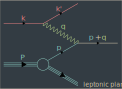
\includegraphics[width=\textwidth]{11dis_diagram.pdf}}
                }
            \end{figure}
        \end{center}
    \end{column}

    \begin{column}{.49\linewidth}
        \vspace{30pt}
        \scriptsize{\textit{
            \ef{Feynmann diagram of DIS.}
            \begin{itemize}
                \vspace{6pt}
                \item
                    The nucleon and quark four-momenta are \eblue{$P$} and \eblue{$p$}, respectively.
                \vspace{6pt}
                \item
                    The initial and final four-momenta of the $e^-$ are \ered{$k$} and \ered{$k'$}.
                \vspace{6pt}
                \item
                    The momentum transferred to the hadron system is \egreen{$q = k - k'$}, conventionally denoted as \egreen{$q^2 = -Q^2$}.
            \end{itemize}
        }}
    \end{column}

    \end{columns}
\end{frame}

